\documentclass[fleqn,10pt]{wlscirep}

\usepackage[utf8]{inputenc}
\usepackage[T1]{fontenc}
%\usepackage[singlelinecheck=off]{caption}

\begin{document}

\section*{Supplementary information to ``Dynamics of non-household contacts during the COVID-19 pandemic in 2020 and 2021 in the Netherlands''}


\renewcommand{\thefigure}{S\arabic{figure}}
\setcounter{figure}{0}
\renewcommand{\thetable}{S\arabic{table}}
\setcounter{table}{0}


\begin{table}[ht]
\centering
\begin{tabular}{rrrrrrrrrrr}
  \hline
year & round & 0-11 & 12-17 & 18-24 & 25-34 & 35-44 & 45-54 & 55-64 & 65+ & total \\ 
  \hline
  2020 &  target &   0 &   0 & 162 & 235 & 225 & 277 & 249 & 352 & 1500 \\ 
  2020 &   1 &   0 &   0 &  88 & 227 & 236 & 308 & 277 & 386 & 1522 \\ 
  2020 &   2 &   0 &   0 &  43 & 176 & 211 & 277 & 255 & 351 & 1313 \\ 
  2020 &   3 &   0 &   0 &  31 & 145 & 168 & 246 & 237 & 316 & 1143 \\ 
  2020 &   4 &   0 &   0 &  30 & 134 & 153 & 223 & 212 & 268 & 1020 \\ 
  2020 &   5 &   0 &   0 &  35 & 131 & 174 & 247 & 231 & 306 & 1124 \\ 
  2020 &   6 &   0 &   0 &  21 & 137 & 174 & 233 & 228 & 318 & 1111 \\ 
  2020 &   7 &   0 &   0 &  20 & 103 & 140 & 215 & 195 & 279 & 952 \\ 
  2020 &   8 &   0 &   0 &  22 & 104 & 142 & 214 & 203 & 284 & 969 \\ 
  \hline
  2021 &   target & 150 & 150 & 248 & 206 & 163 & 184 & 161 & 238 & 1500 \\ 
  2021 &   1 & 137 & 145 & 239 & 202 & 158 & 180 & 158 & 232 & 1451 \\ 
  2021 &   2 & 126 & 126 & 139 & 175 & 136 & 177 & 176 & 257 & 1312 \\ 
  2021 &   3 & 107 & 115 & 174 & 175 & 136 & 149 & 128 & 187 & 1171 \\ 
  2021 &   4 &  99 & 104 & 112 & 157 & 110 & 125 & 142 & 213 & 1062 \\ 
  2021 &   5 &  81 &  95 &  94 & 127 &  89 & 132 & 127 & 197 & 942 \\ 
  2021 &   6 &  87 &  75 & 110 & 151 & 126 & 118 &  95 &  92 & 854 \\ 
  2021 &   7 &  73 &  67 &  64 & 126 &  85 &  93 & 115 & 143 & 766 \\ 
  2021 &   8 &  68 &  76 &  80 & 133 & 102 & 123 &  78 & 103 & 763 \\ 
  2021 &   9 &  49 &  67 &  78 & 117 &  94 &  86 &  61 &  64 & 616 \\ 
  2021 &  10 &  40 &  65 &  65 & 104 &  89 &  96 &  71 &  31 & 561 \\ 
  2021 &  11 & 116 & 154 & 195 & 205 & 160 & 198 & 167 & 260 & 1455 \\ 
  2021 &  12 & 107 & 133 & 178 & 194 & 155 & 160 & 142 & 208 & 1277 \\ 
  2021 &  13 &  96 & 115 & 124 & 163 & 121 & 154 & 152 & 233 & 1158 \\ 
  2021 &  14 &  84 &  98 &  85 & 143 & 117 & 134 & 140 & 228 & 1029 \\ 
  2021 &  15 &  77 &  86 &  84 & 135 & 117 & 123 & 113 & 188 & 923 \\ 
  2021 &  16 &  71 &  74 &  50 & 117 &  98 & 117 & 112 & 192 & 831 \\ 
  2021 &  17 &  59 &  82 &  48 & 115 & 103 & 130 & 119 & 106 & 762 \\ 
  2021 &  18 &  55 &  69 &  41 &  90 &  65 &  72 & 105 & 181 & 678 \\ 
  2021 &  19 &  64 &  56 &  43 &  90 &  79 &  73 &  70 & 201 & 676 \\ 
  2021 &  20 &  47 &  81 &  41 &  86 &  84 & 100 &  87 & 160 & 686 \\ 
   \hline
\end{tabular}
\caption{\label{tab:part_round}Number of participants per survey round of study series in 2020 and 2021 in eight age groups. The target number of participants was to be achieved in round 1 in 2020, and in rounds 1 and 11 in 2021.} 
\end{table}

\begin{figure}[ht]
\centering
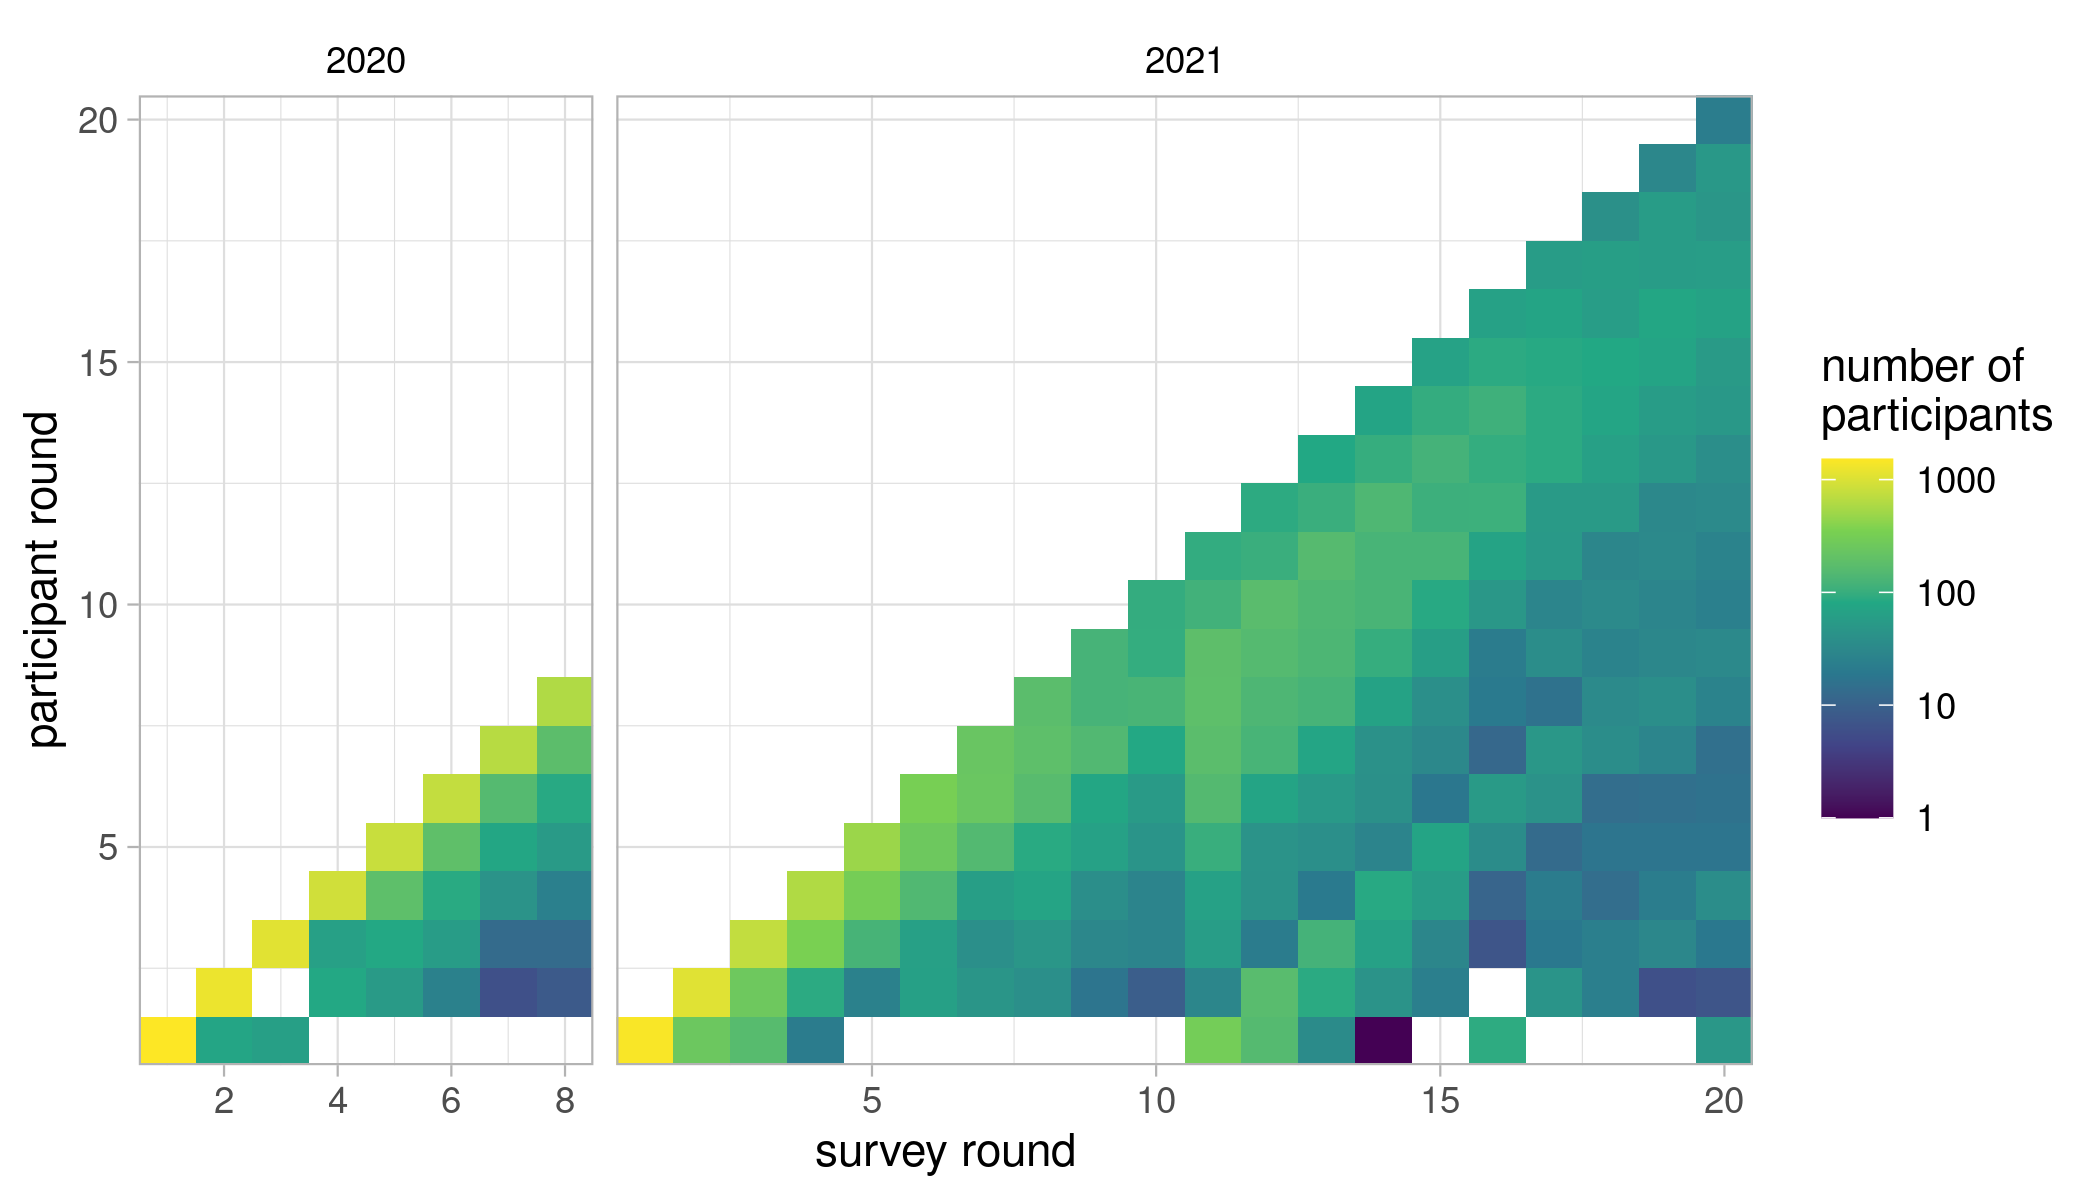
\includegraphics[width=\linewidth]{../figures/participant_rounds.png}
\caption{Number of participants by survey round and participant round (i.e. the n\textsuperscript{th} time a participant participated). Series 2020 (left) consisted of 8 rounds, series 2021 (right) consisted of 20 rounds. Most participants participated for the first time the start of the series, but some also started during the study period. The panel was supplemented to the target population in round 11 of series 2021.}
\label{fig:part_round}
\end{figure}



\begin{table}[ht]
\centering
\begin{tabular}{rrlrrrrl}
  \hline
series & age\_group & Variable & Estimate & Std. Error & t value & p-value & \\ 
  \hline
  2020 & 18-64 & (Intercept) & -0.23 & 0.06 & -3.85 & $<$ 0.001 & *** \\ 
  2020 & 18-64 & part\_vaccTRUE & 0.00 & 0.00 &  &  &  \\ 
  2020 & 18-64 & part\_elevated\_riskTRUE & -0.03 & 0.08 & -0.40 & 0.69 &  \\ 
  2020 & 18-64 & weekendTRUE & -0.21 & 0.06 & -3.67 & $<$ 0.001 & *** \\ 
  2020 & 18-64 & holidayTRUE & 0.07 & 0.10 & 0.72 & 0.47 &  \\ 
  2020 & 18-64 & Deviance explained & 0.16 &  &  &  &  \\ 
  \hline
  2020 & 65+ & (Intercept) & 0.03 & 0.13 & 0.27 & 0.79 &  \\ 
  2020 & 65+ & part\_vaccTRUE & 0.00 & 0.00 &  &  &  \\ 
  2020 & 65+ & part\_elevated\_riskTRUE & 0.25 & 0.12 & 2.05 & 0.04 & * \\ 
  2020 & 65+ & weekendTRUE & -0.32 & 0.08 & -3.89 & $<$ 0.001 & *** \\ 
  2020 & 65+ & holidayTRUE & -0.08 & 0.11 & -0.70 & 0.48 &  \\ 
  2020 & 65+ & Deviance explained & 0.14 &  &  &  &  \\ 
  \hline
  2021 & 0-17 & (Intercept) & -0.81 & 0.08 & -9.91 & $<$ 0.001 & *** \\ 
  2021 & 0-17 & part\_vaccTRUE & 0.12 & 0.19 & 0.64 & 0.52 &  \\ 
  2021 & 0-17 & part\_elevated\_riskTRUE & -0.15 & 0.27 & -0.56 & 0.57 &  \\ 
  2021 & 0-17 & weekendTRUE & -0.67 & 0.08 & -8.35 & $<$ 0.001 & *** \\ 
  2021 & 0-17 & holidayTRUE & -0.20 & 0.10 & -2.04 & 0.04 & * \\ 
  2021 & 0-17 & Deviance explained & 0.17 &  &  &  &  \\ 
  \hline
  2021 & 18-64 & (Intercept) & -0.92 & 0.06 & -16.00 & $<$ 0.001 & *** \\ 
  2021 & 18-64 & part\_vaccTRUE & 0.09 & 0.07 & 1.31 & 0.19 &  \\ 
  2021 & 18-64 & part\_elevated\_riskTRUE & -0.13 & 0.08 & -1.72 & 0.08 & . \\ 
  2021 & 18-64 & weekendTRUE & -0.27 & 0.05 & -5.88 & $<$ 0.001 & *** \\ 
  2021 & 18-64 & holidayTRUE & 0.06 & 0.06 & 0.94 & 0.35 &  \\ 
  2021 & 18-64 & Deviance explained & 0.19 &  &  &  &  \\ 
  \hline
  2021 & 65+ & (Intercept) & -0.82 & 0.15 & -5.51 & $<$ 0.001 & *** \\ 
  2021 & 65+ & part\_vaccTRUE & 0.08 & 0.19 & 0.40 & 0.69 &  \\ 
  2021 & 65+ & part\_elevated\_riskTRUE & -0.10 & 0.11 & -0.89 & 0.37 &  \\ 
  2021 & 65+ & weekendTRUE & -0.44 & 0.08 & -5.65 & $<$ 0.001 & *** \\ 
  2021 & 65+ & holidayTRUE & 0.04 & 0.10 & 0.42 & 0.68 &  \\ 
  2021 & 65+ & Deviance explained & 0.16 &  &  &  &  \\ 
   \hline
\end{tabular}
\caption{\label{tab:fixed_effects}Results for fixed effects of generalised additive model, by series (2020, 2021) and age group (0-17, 16-64, 65+). Included fixed effects are participant vaccination status (part\_vacc), participant risk status (part\_elevated\_risk), weekend and holiday. Holidays include general holidays and school holidays. The last row of each section refers to the explained deviance.
Significance levels: *** (p-value $<$ 0.001), ** (p-value $<$ 0.01), * (p-value $<$ 0.05), . (p-value $<$ 0.1) } 
\end{table}


\begin{figure}[ht]
\centering
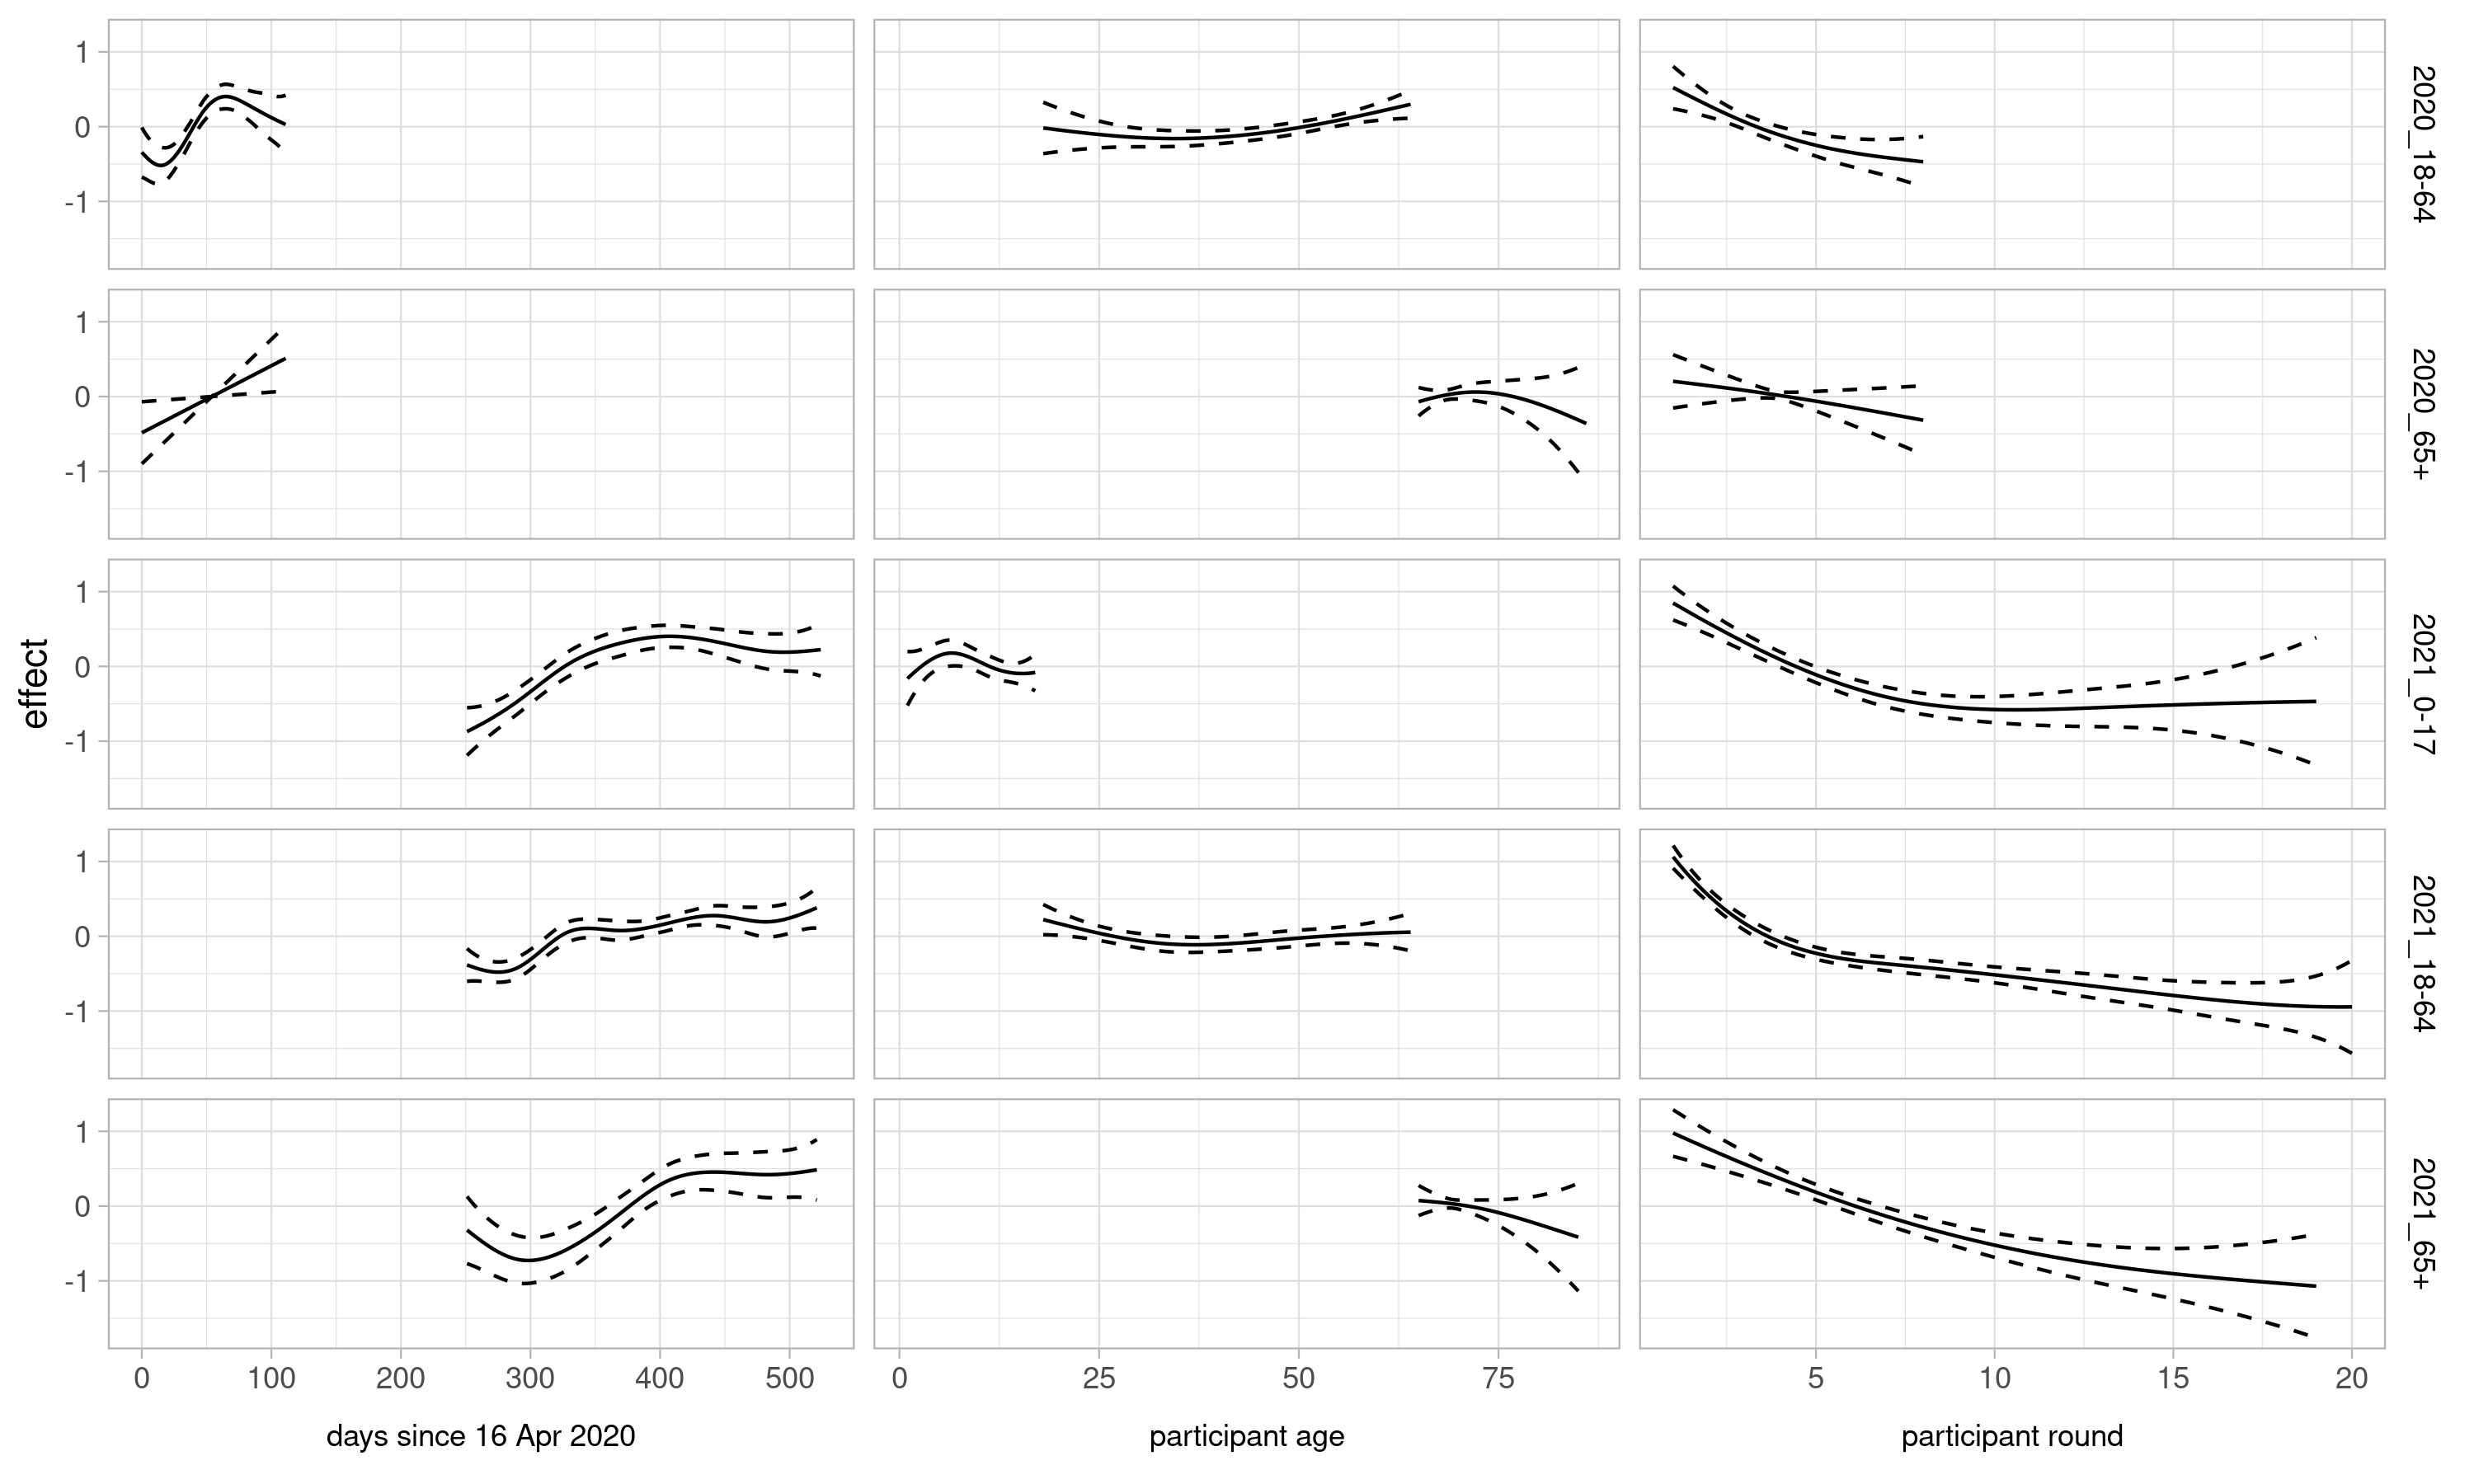
\includegraphics[width=\linewidth]{../figures/results_splines.png}
\caption{Results for non-stationary fixed effects of generalised additive model, by series (2020, 2021) and age group (0-17, 16-64, 65+). Calendar time (expressed as days since first survey), participant age, and participant round (i.e. the n\textsuperscript{th} time a participant participated) are included as cubic splines. Shown are the fitted splines (solid lines) $\pm$ the standard error (dashed lines).}
\label{fig:splines}
\end{figure}


\end{document}